\section{Sliding Windows and Data Parallelization}

\begin{figure*}[t]
\centering
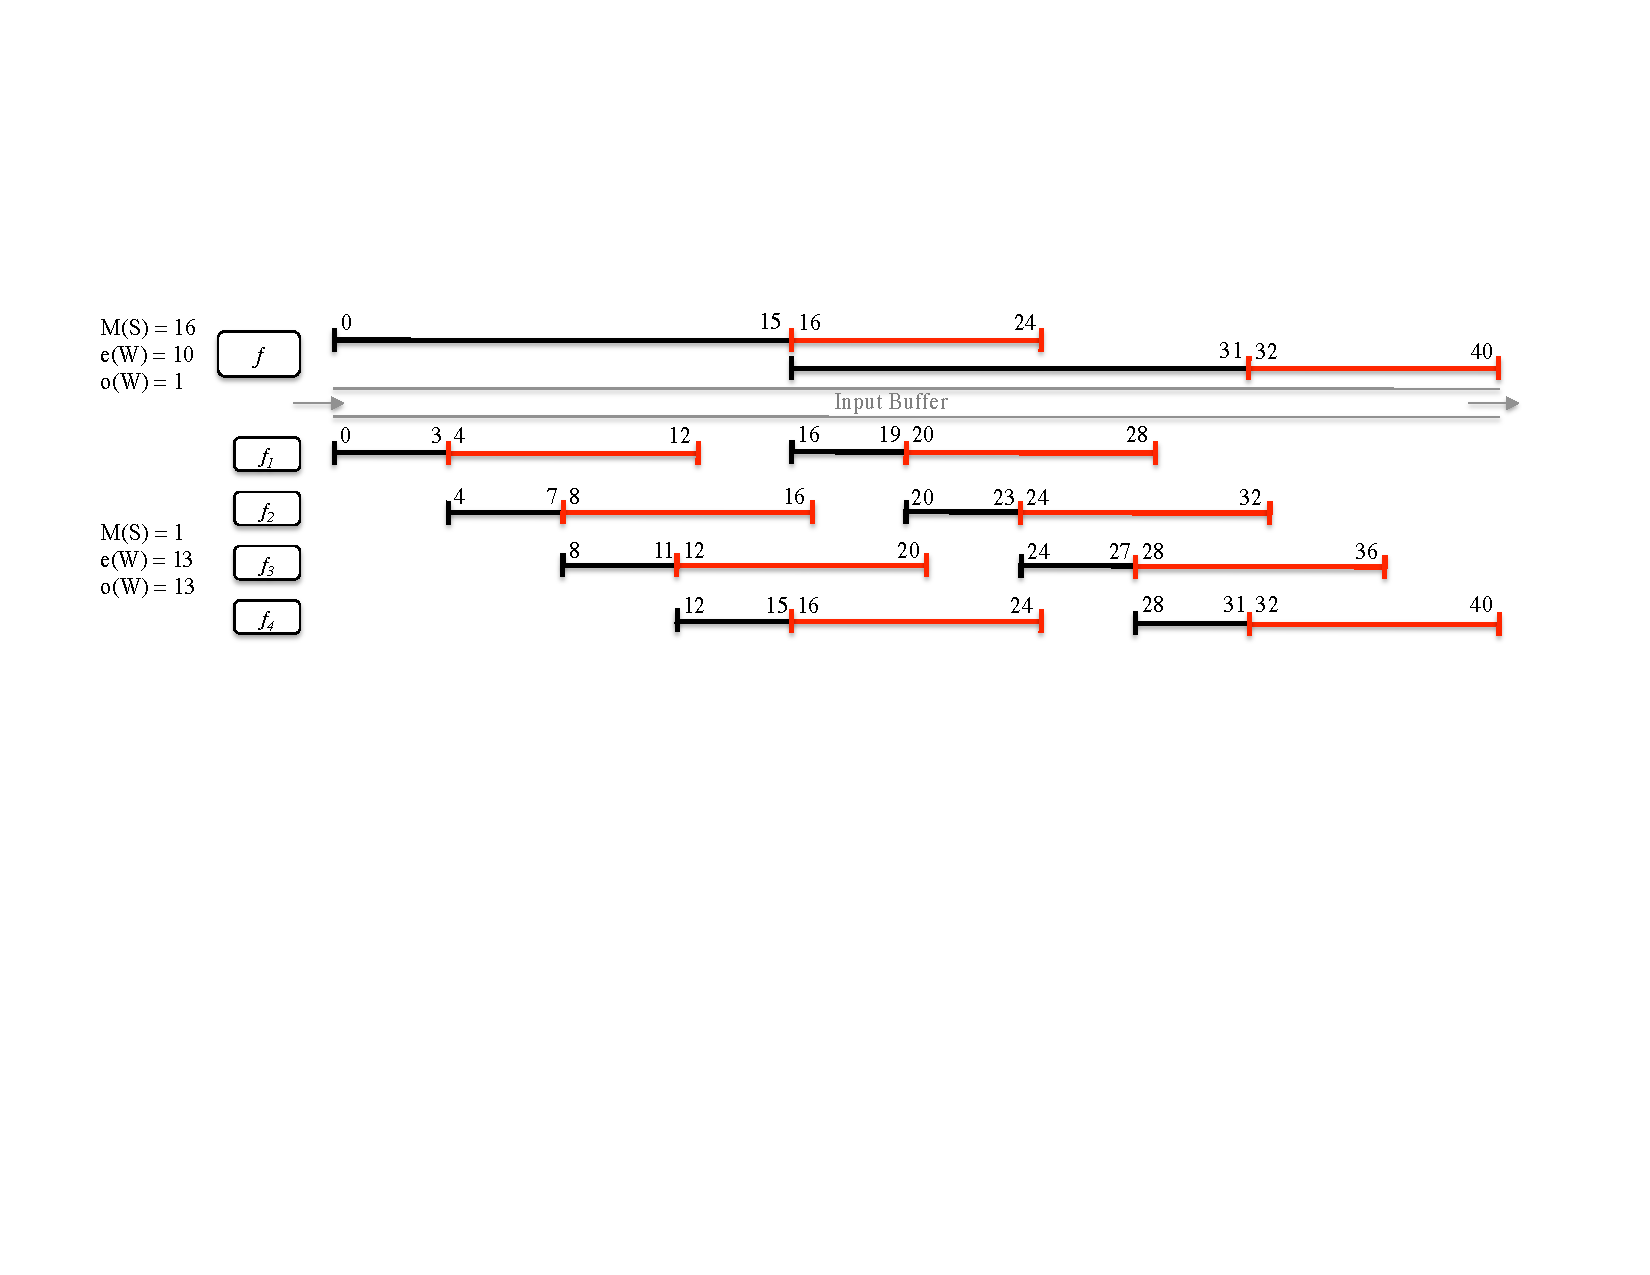
\includegraphics[width=6.0in]{figures/fission-sharing.pdf}
\caption[An example of the sharing required by fission.]  { An
  example of the duplication of items required by fission.  Filter $f$
  is fissed by 4 into $f_1$ - $f_4$.  Two steady-states of the item
  indices required for both $f$ and the fission products are shown.
  Item indices that are inspected but not dequeued are in red.  For the
  fission products, it is required to duplicate 1 out of 4 items to
  all 4 filters, and the remaining 3 items are duplicated to 3
  filters.  Notice that the number of items inspected by the fission
  products is the same as $f$, but the total number of items dequeued 
per steady-state is split across the $f_i$s.
\label{fig:fission-sharing}}
\end{figure*}


\begin{figure*}
\centering
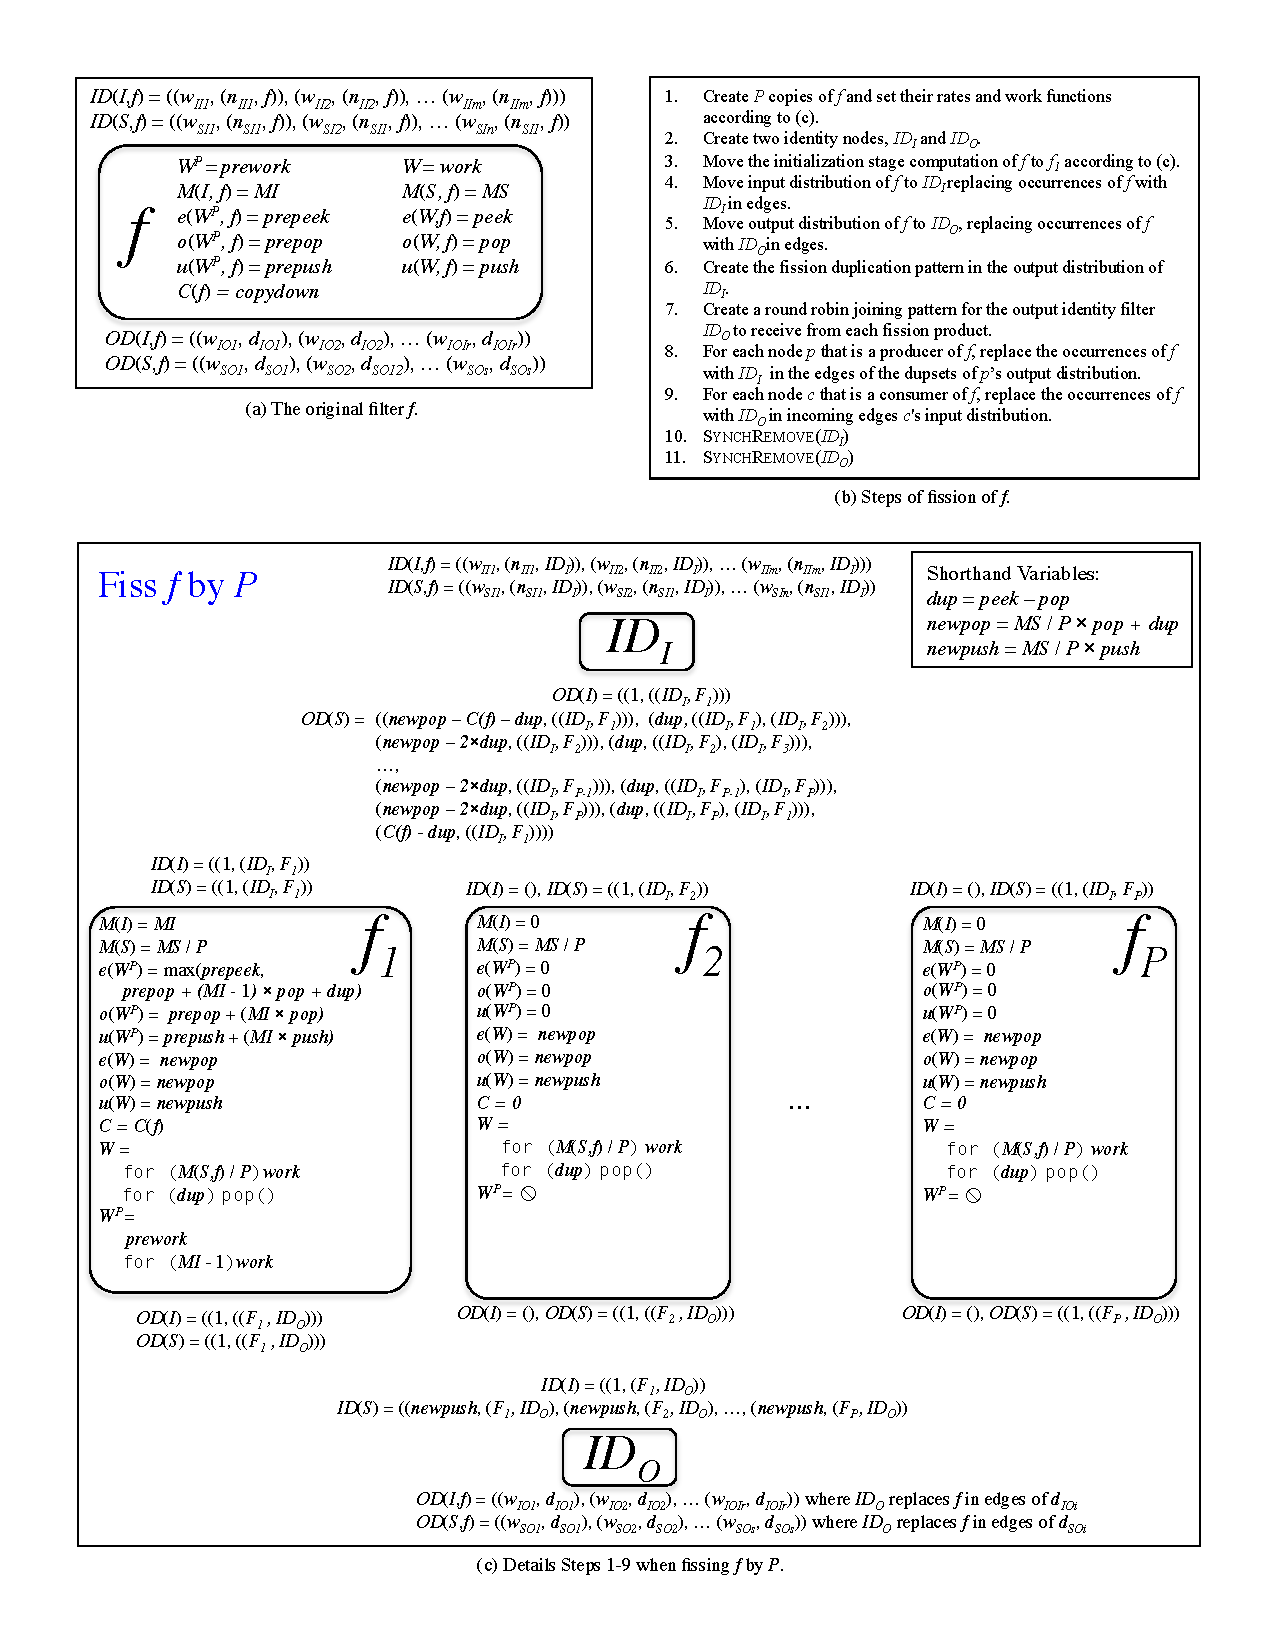
\includegraphics[width=\textwidth]{figures/general-fission.pdf}
\caption[Fission of a node in the general stream graph.]{Fission of a
  node $f$ by $P$ in the general stream
  graph.\label{fig:general-fission}}
\end{figure*}


Automatic data parallelization is possible if the compiler can reason
about the sharing requirement of the sliding window filter.  When a
sliding window filter is parallelized via the process of fission, the
window state inherent between iterations is transformed into the
communication of shared items to multiple products of the filter.
Figure~\ref{fig:fission-sharing} gives an example of the sharing
requirement between fission products for a fission application.
Previous work implements fission of sliding window filters via
duplication of all input items to all fission products and decimation
of unneeded items at each product filter~\cite{streamit-asplos}.  We
call this technique {\it DupDec}. If each product is mapped to a
distinct core, the replication of items requires inter-core
communication.

The efficiency of DupDec depends on the application being mapped and
the communication mechanism of the target.  Two of our benchmarks
include significant amounts of {\it unnecessary} duplication in the
steady-state when DupDec is utilized by the techniques described
in~\cite{gordon-asplos06}:

\begin{itemize}
\item ChannelVocoder: 5,200 of 13,336 total items (38\%)
\item FMRadio: 1,108 of 1,808 total items (61\%) 
\end{itemize}

This is because there is little overlap in the sliding windows of
product filters for these benchmarks, and DupDec duplicates each input
item to all products. Conversely, our techniques will always avoid
unnecessary duplication of input items.

Even without unnecessarily duplication of items, inter-core
communication as a result of fission accounts for a large percentage
of the total items communicated between filters of an application.
ChannelVocoder has 48\% of total communication as inter-core
communication caused by fission, Filterbank 50\%, and FMRadio 93\%.
Employing our techniques, for our benchmarks, we are able to reduce
the percentage of inter-core communication by altering the steady
state.

In the general case, when fissing a filter that peeks, i.e., a filter
$f$ with $e(W, f) - o(W, f) = \mt{dup}_f < C(f) > 0$, by $P$, the producers
of $f$ need to duplicate output items to an average of:
{
\ninepoint
\[ \max \left ( 1 + \frac{C(f)}{M(S, f) \cdot o(W, f) / P}, P \right )\]
}
\noindent fission products of $f$.  Figure~\ref{fig:fission-sharing}
gives an example of the required sharing for a fission application.
The filter $f$ is duplicated 4 ways, has $C(f) = 9$, $o(W, f) = 1$,
and $M(S, f) = 16$.  From the above formula, each item is duplicated
to an average of $3.25$ fission products.

% Figure~\ref{fig:fir-nopeeking} gives an implementation of
% an FIR filter in the StreamIt programming language without using the
% language's peeking support.  This implementation requires
% sophisticated compiler analyses in order to parallelize.
% The programmer is forced to use a circular buffer to represent the
% sliding window of the FIR computation.  Modulo operations are used in
% the address calculation for the circular buffer.  Modulo operations
% are typically not handled by array dependence analysis frameworks.  So
% in the presence of modulo operations, the compiler must conservatively
% assume that each read and write can access any location in the array.
